\documentclass[a4paper, 14pt]{extarticle}
\usepackage[russian,english]{babel}
\usepackage[T1]{fontenc}
\usepackage{fontspec}
\usepackage{indentfirst}
\usepackage{enumitem}
\usepackage{graphicx}
\usepackage[
  left=20mm,
  right=10mm,
  top=20mm,
  bottom=20mm
]{geometry}
\usepackage{parskip}
\usepackage{titlesec}
\usepackage{xurl}
\usepackage{hyperref}
\usepackage{float}
\usepackage[
  figurename=Рисунок,
  labelsep=endash,
  justification=centering
]{caption}
\usepackage[outputdir=build, newfloat]{minted}
\usepackage{chngcntr}

\hypersetup{
  colorlinks=true,
  linkcolor=black,
  filecolor=blue,
  urlcolor=blue,
}

\renewcommand*{\labelitemi}{---}
\setmainfont{Times New Roman}
\setmonofont{JetBrains Mono}[
  SizeFeatures={Size=11},
]

\newenvironment{code}{\captionsetup{type=figure}}{}
\BeforeBeginEnvironment{code}{\bigskip}
\AfterEndEnvironment{code}{\bigskip}

\setminted{
  fontsize=\footnotesize,
}

\setlength{\parskip}{6pt}

\setlength{\parindent}{1.25cm}
\setlist[itemize]{itemsep=0em,topsep=0em,parsep=0em,partopsep=0em,leftmargin=2.0cm,wide}
\setlist[enumerate]{itemsep=0em,topsep=0em,parsep=0em,partopsep=0em,leftmargin=2.0cm,wide}

\renewcommand{\thesection}{\indent\arabic{section}.}
\renewcommand{\thesubsection}{\indent\thesection\arabic{subsection}.}
\renewcommand{\thesubsubsection}{\indent\thesubsection\arabic{subsubsection}.}

\titleformat{\section}{\normalfont\bfseries}{\thesection}{0.5em}{}
\titleformat{\subsection}{\normalfont\bfseries}{\thesubsection}{0.5em}{}
\titleformat{\subsubsection}{\normalfont\bfseries}{\thesubsubsection}{0.5em}{}

\titleformat*{\section}{\normalfont\bfseries}
\titleformat*{\subsection}{\normalfont\bfseries}
\titleformat*{\subsubsection}{\normalfont\bfseries}

\titlespacing{\section}{\parindent}{\parskip}{\parskip}
\titlespacing{\subsection}{\parindent}{\parskip}{\parskip}
\titlespacing{\subsubsection}{\parindent}{\parskip}{\parskip}

\begin{document}

\begin{titlepage}
  \vspace{0pt plus2fill}
  \noindent

  \vspace{0pt plus6fill}
  \begin{center}
    {
    \bfseries
    Министерство науки и высшего образования Российской Федерации
    {
    \scriptsize
    ФЕДЕРАЛЬНОЕ ГОСУДАРСТВЕННОЕ АВТОНОМНОЕ ОБРАЗОВАТЕЛЬНОЕ УЧРЕЖДЕНИЕ ВЫСШЕГО
    ОБРАЗОВАНИЯ
    }
    «Национальный исследовательский университет ИТМО»

    (Университет ИТМО)

    \begin{minipage}[t]{0.42\textwidth}
      \vspace*{0pt}
      \begin{flushright}
        Факультет

        Образовательная программа
      \end{flushright}
    \end{minipage}
    \begin{minipage}[t]{0.57\textwidth}
      \vspace*{0pt}
      \begin{flushright}
        Инфокоммуникационных технологий

        11.03.02 Программирование в инфокоммуникационных системах
      \end{flushright}
    \end{minipage}
    }

    \vspace{0pt plus5fill}

    \LARGE{
      ОТЧЕТ

      по лабораторной работе 1

      по дисциплине \textbf{<<Разработка баз данных>>}
    }
  \end{center}

  \vspace{0pt plus4fill}
  \begin{flushright}
    Выполнил: \textbf{студент группы K33211 Швалов Д. А.}

    Проверил: \textbf{ст. преподаватель Осетрова И.С.}
  \end{flushright}

  \vspace{0pt plus8fill}
  \begin{center}
    Санкт-Петербург

    2024
  \end{center}
\end{titlepage}

\setcounter{page}{2}

\linespread{1.5}
\renewcommand{\baselinestretch}{1.5}

\section*{\large{Лабораторная работа №1 <<Создание БД и схемы>>}}

\section{Цель работы}

Научиться создавать, изменять, удалять базы данных и схемы СУБД Microsoft SQL
Server в интегрированной среде управления базами данных Microsoft SQL Server
Management Studio (SSMS).

\section{Задачи, решаемые при выполнении работы}

\begin{enumerate}[leftmargin=*]
  \item Создание учебной базы данных в среде SSMS.
  \item Создание сценария базы данных из SSMS.
  \item Удаление учебной базы данных в SSMS.
  \item Создание учебной базы данных в Query Editor.
  \item Создание схемы в SSMS.
  \item Создание схемы в Query Editor.
\end{enumerate}

\section{Объект исследования}

Базы данных и схемы СУБД Microsoft SQL Server.

\section{Исходные данные}

Интегрированная среда управления базами данных Microsoft SQL Server Management Studio (SSMS).

\section{Выполнение работы}

\subsection{Первая задача}

\subsubsection{Предварительная настройка базы данных}

На панели <<Object Explorer>> был выбран узел <<Databases>>. В контекстном меню
был выбран пункт <<New Database>>. После этого открылось окно, которое показано
на рисунке \ref{fig:task-1/step-1.png}. В поле <<Database name>> было введено
название <<ApressFinancial>>. Поле <<Owner>> было оставлено без изменений.

\begin{figure}[H]
  \centering
  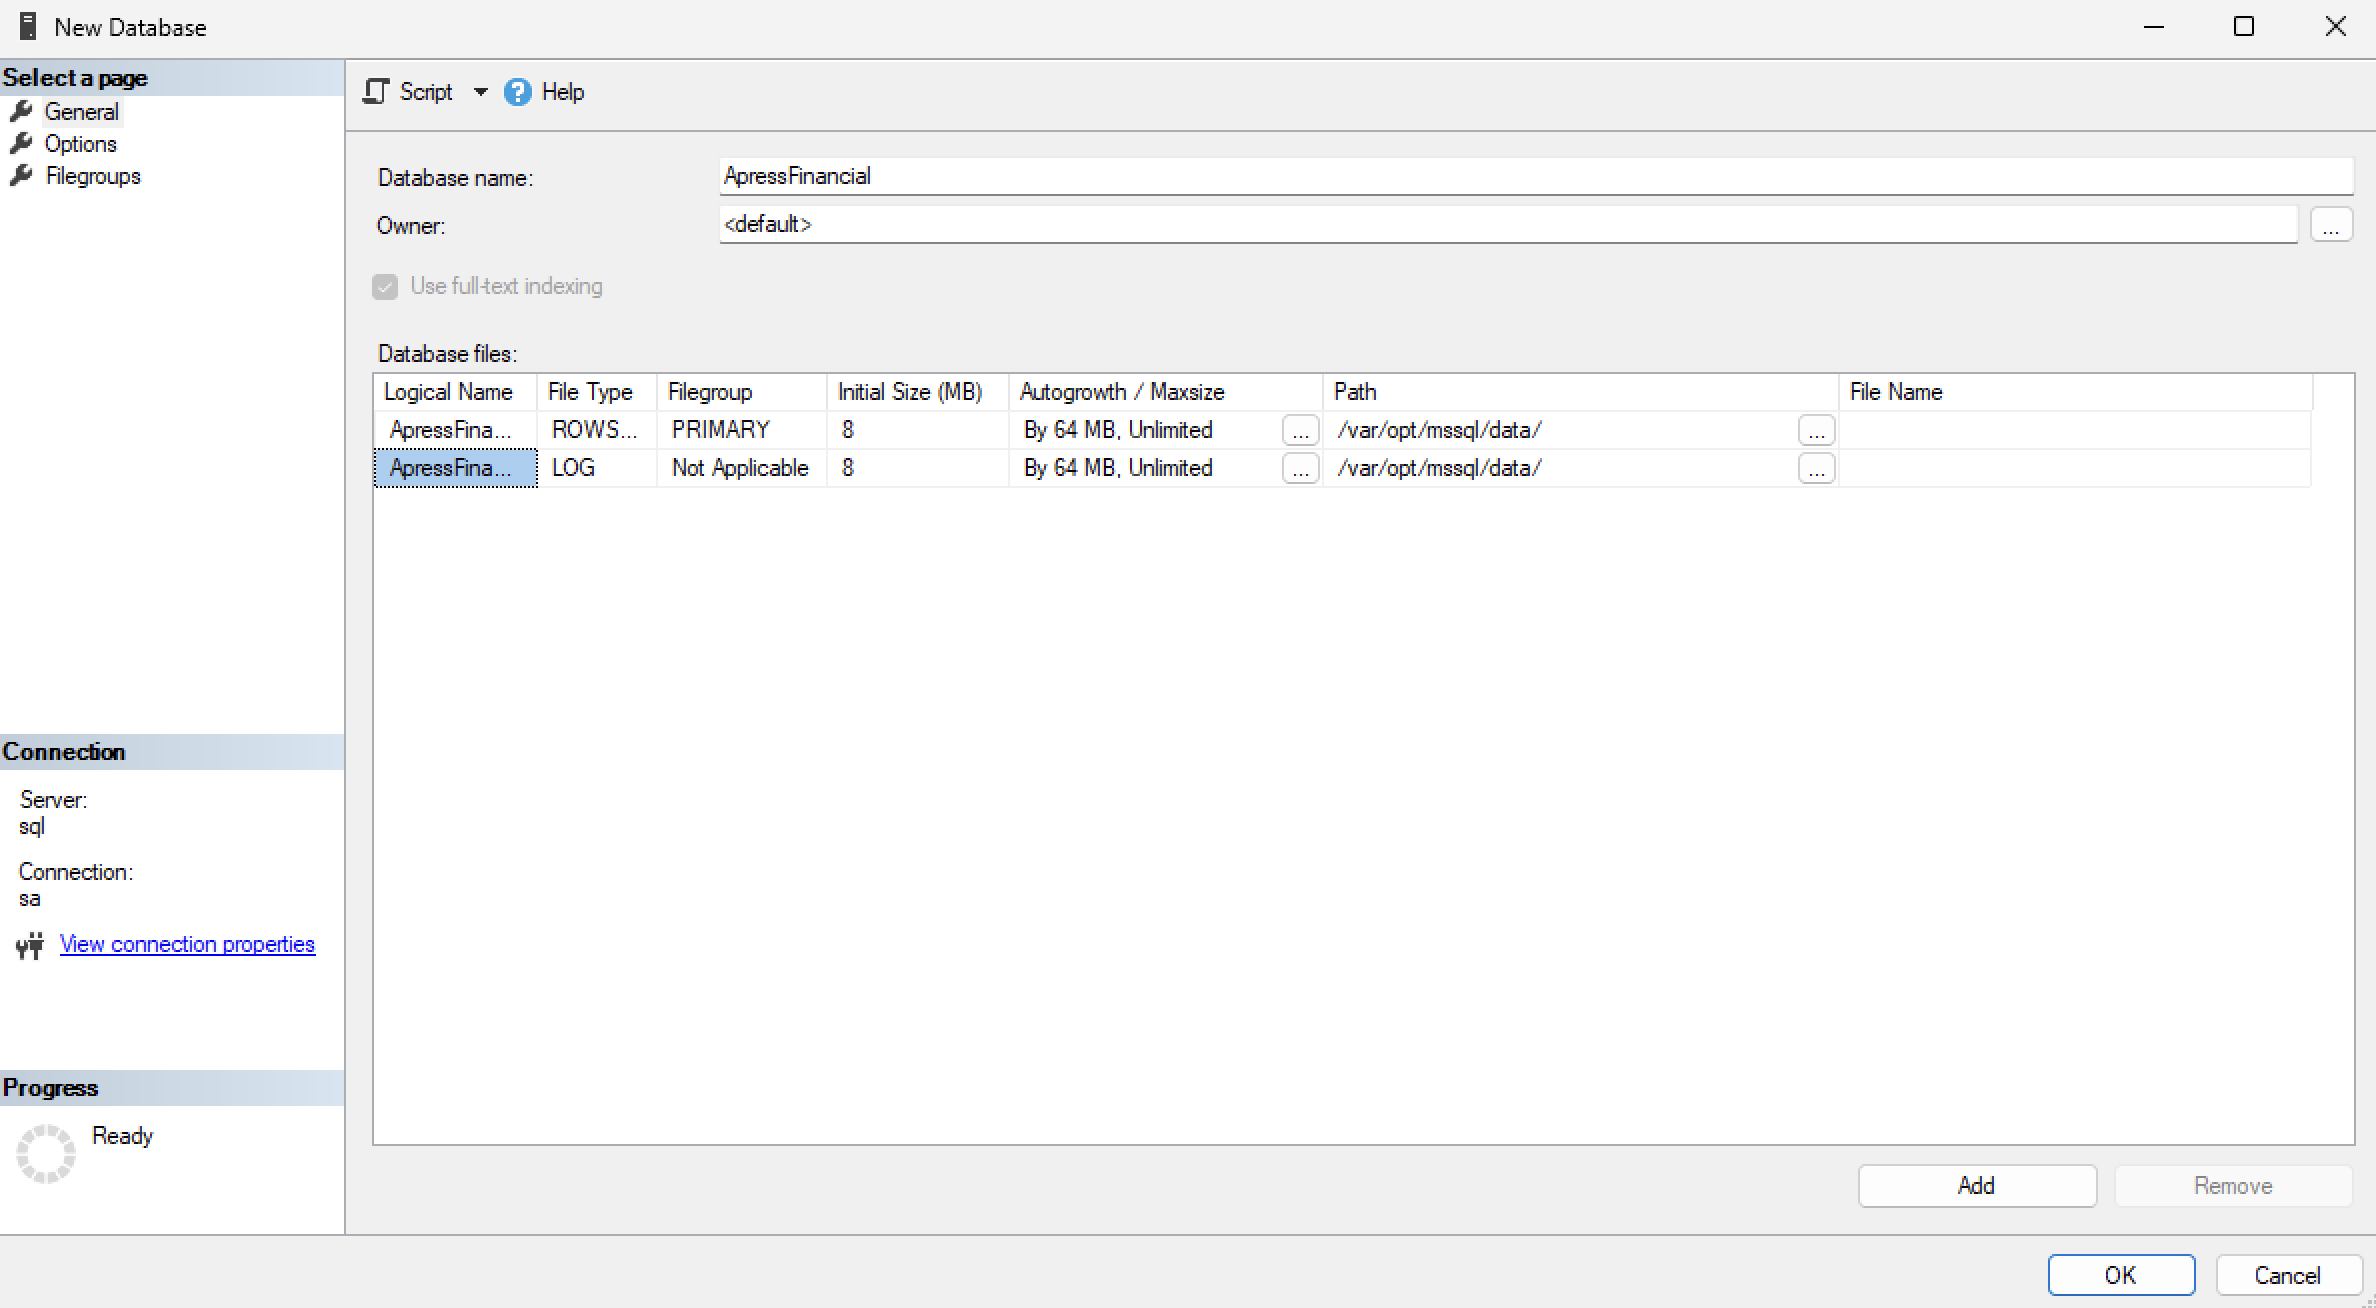
\includegraphics[width=\textwidth]{images/task-1/step-1.png}
  \caption{Создание новой базы данных}
  \label{fig:task-1/step-1.png}
\end{figure}

\subsubsection{Создание вторичного файла данных}

С помощью кнопки <<Add>> был добавлен вторичный файл данных с названием (поле
<<Logical Name>>) равным <<ApressFinancial\_act>>. В столбце <<File Type>> было
выбрано значение <<ROWS Data>>, что означает, что добавляемый файл будет
является файлом данных, а не файлом журнала. В результате в окне появилась еще
одна строка, показанная на рисунке \ref{fig:task-1/step-2.png}.

\begin{figure}[H]
  \centering
  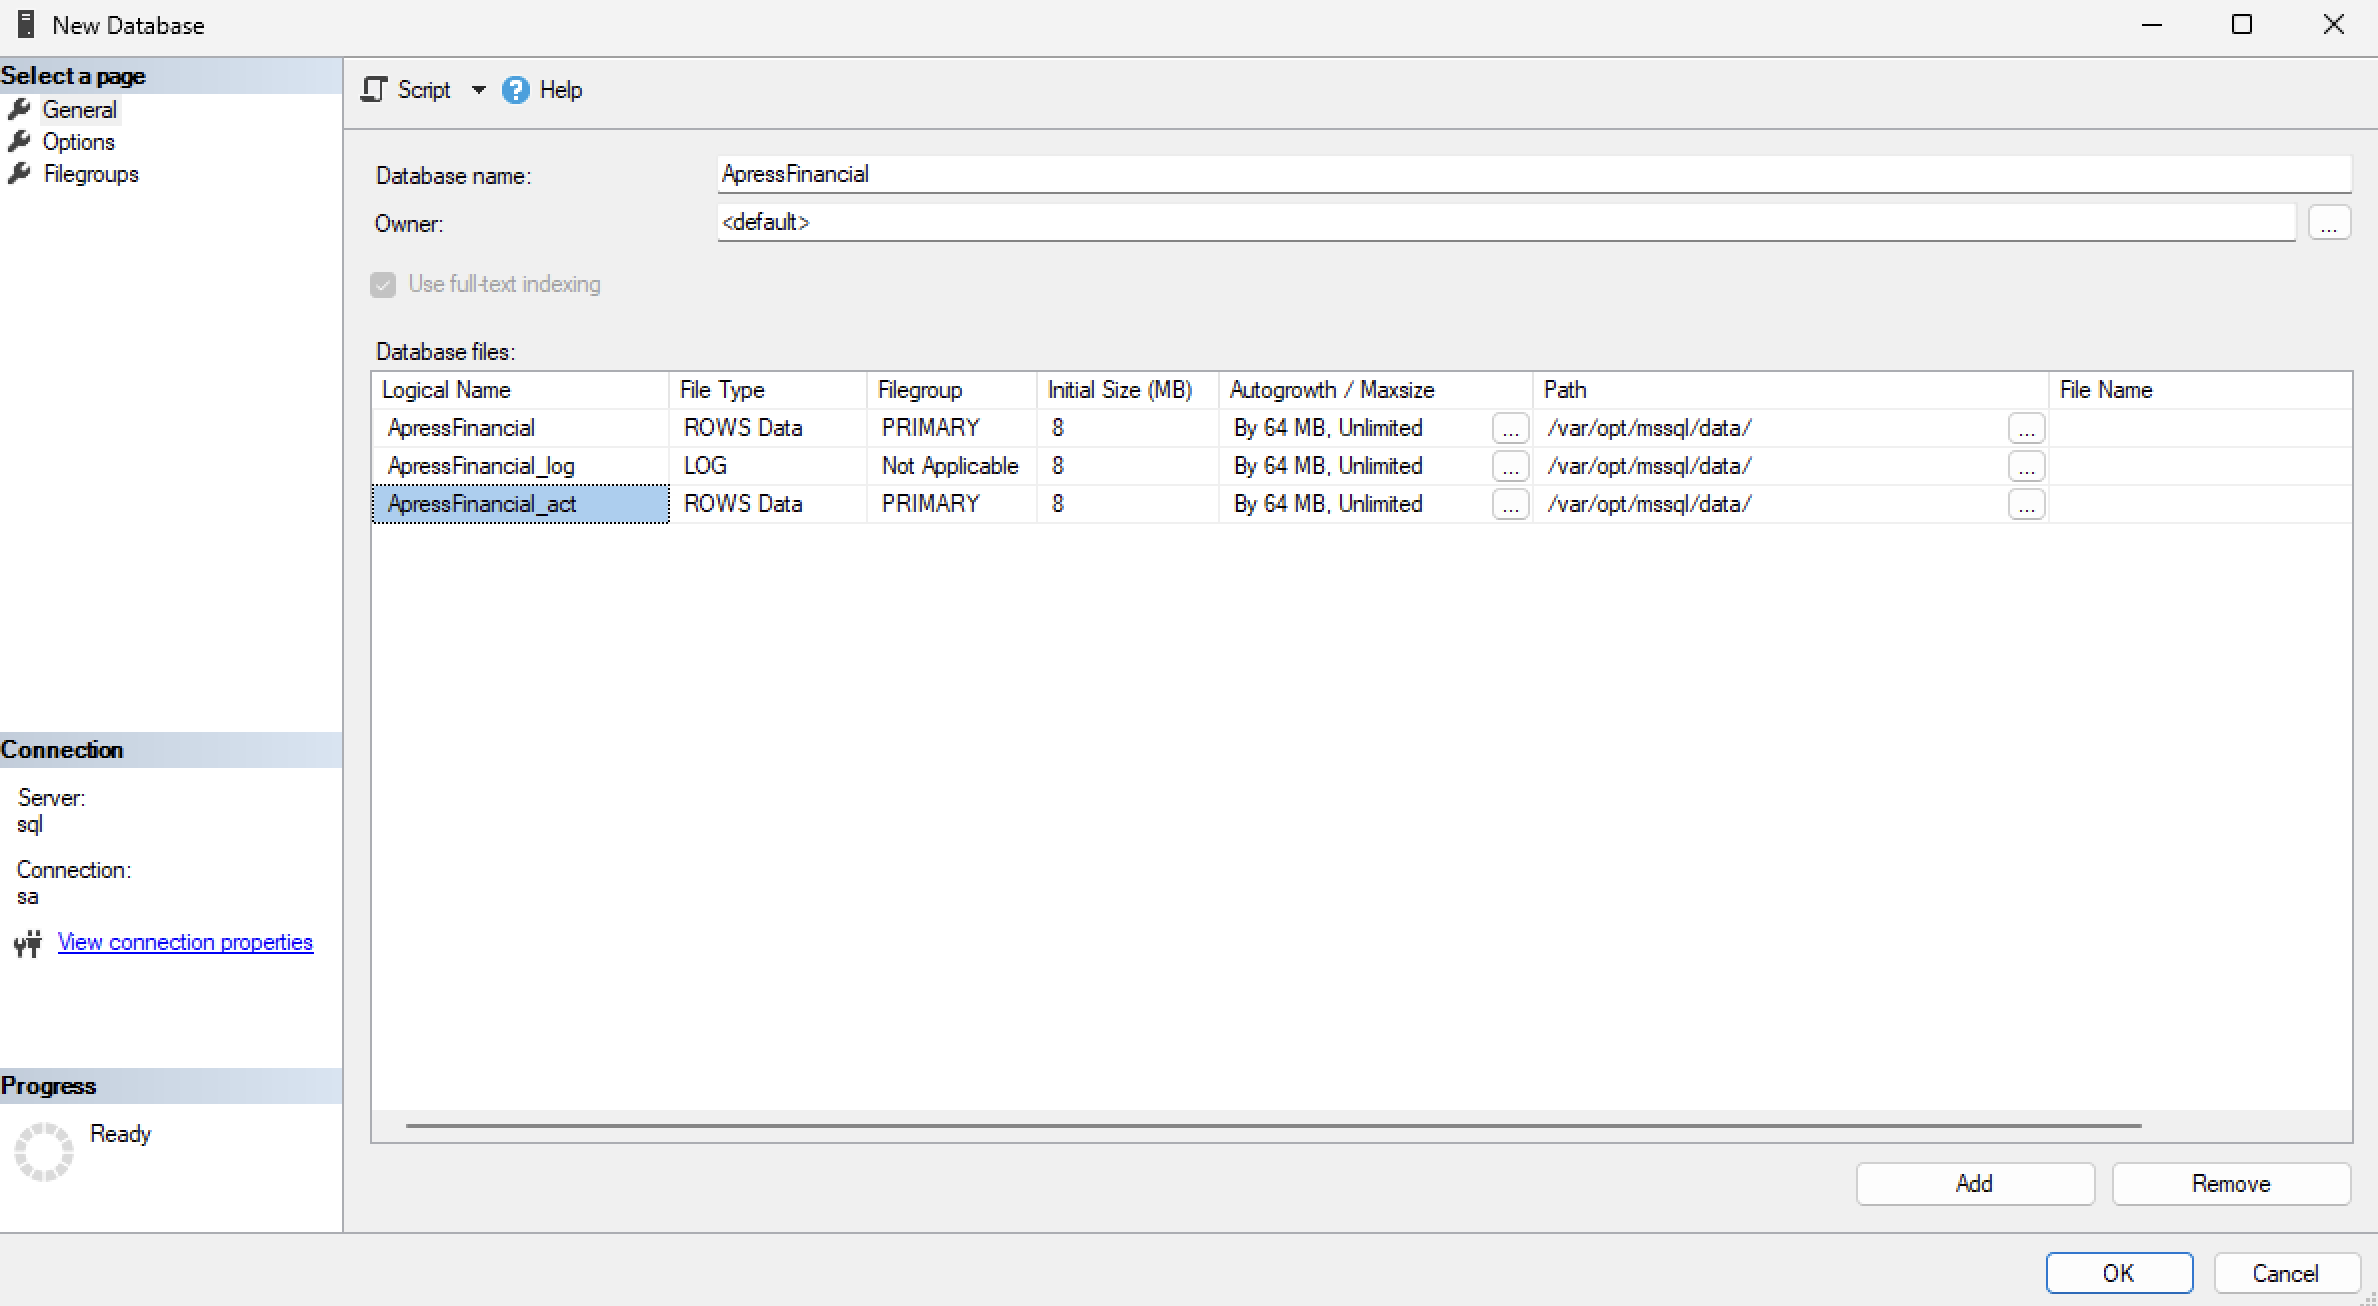
\includegraphics[width=\textwidth]{images/task-1/step-2.png}
  \caption{Создание вторичного файла данных}
  \label{fig:task-1/step-2.png}
\end{figure}

\subsubsection{Настройка вторичного файла данных}

Для добавленного файла данных был настроен параметр <<Filegroup>>. В окне,
показанном на рисунке \ref{fig:task-1/step-3.png} в поле <<Name>> было введено
значение <<SECONDARY>>, а также проставлено флажок <<Default>>.

\begin{figure}[H]
  \centering
  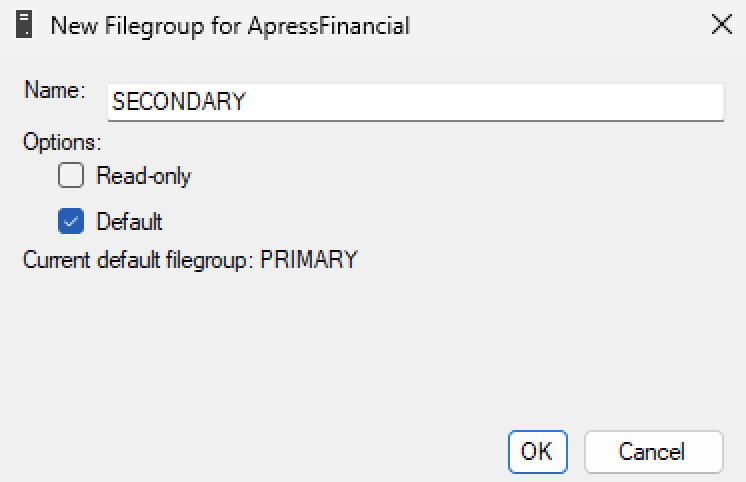
\includegraphics[width=0.6\textwidth]{images/task-1/step-3.png}
  \caption{Настройка параметра <<Filegroup>>}
  \label{fig:task-1/step-3.png}
\end{figure}

\subsubsection{Настройка параметров базы данных}

В соответствии с заданием, для базы данных были установлены следующие параметры
Automatic:
\begin{itemize}
  \item Auto Close в значение True;
  \item Auto Create Statistics в значение True;
  \item Auto Shrink в значение False;
  \item Auto Update Statistics в значение True;
  \item Auto Update Statistics Asynchronously в значение True.
\end{itemize}

В качестве параметров сортировки (Collation), модели восстановления (Recovery
model) и уровня совместимости (Compatibility level) были оставлены значения по
умолчанию.

Настроенные параметры показаны на рисунке \ref{fig:task-1/step-4.png}.

\begin{figure}[H]
  \centering
  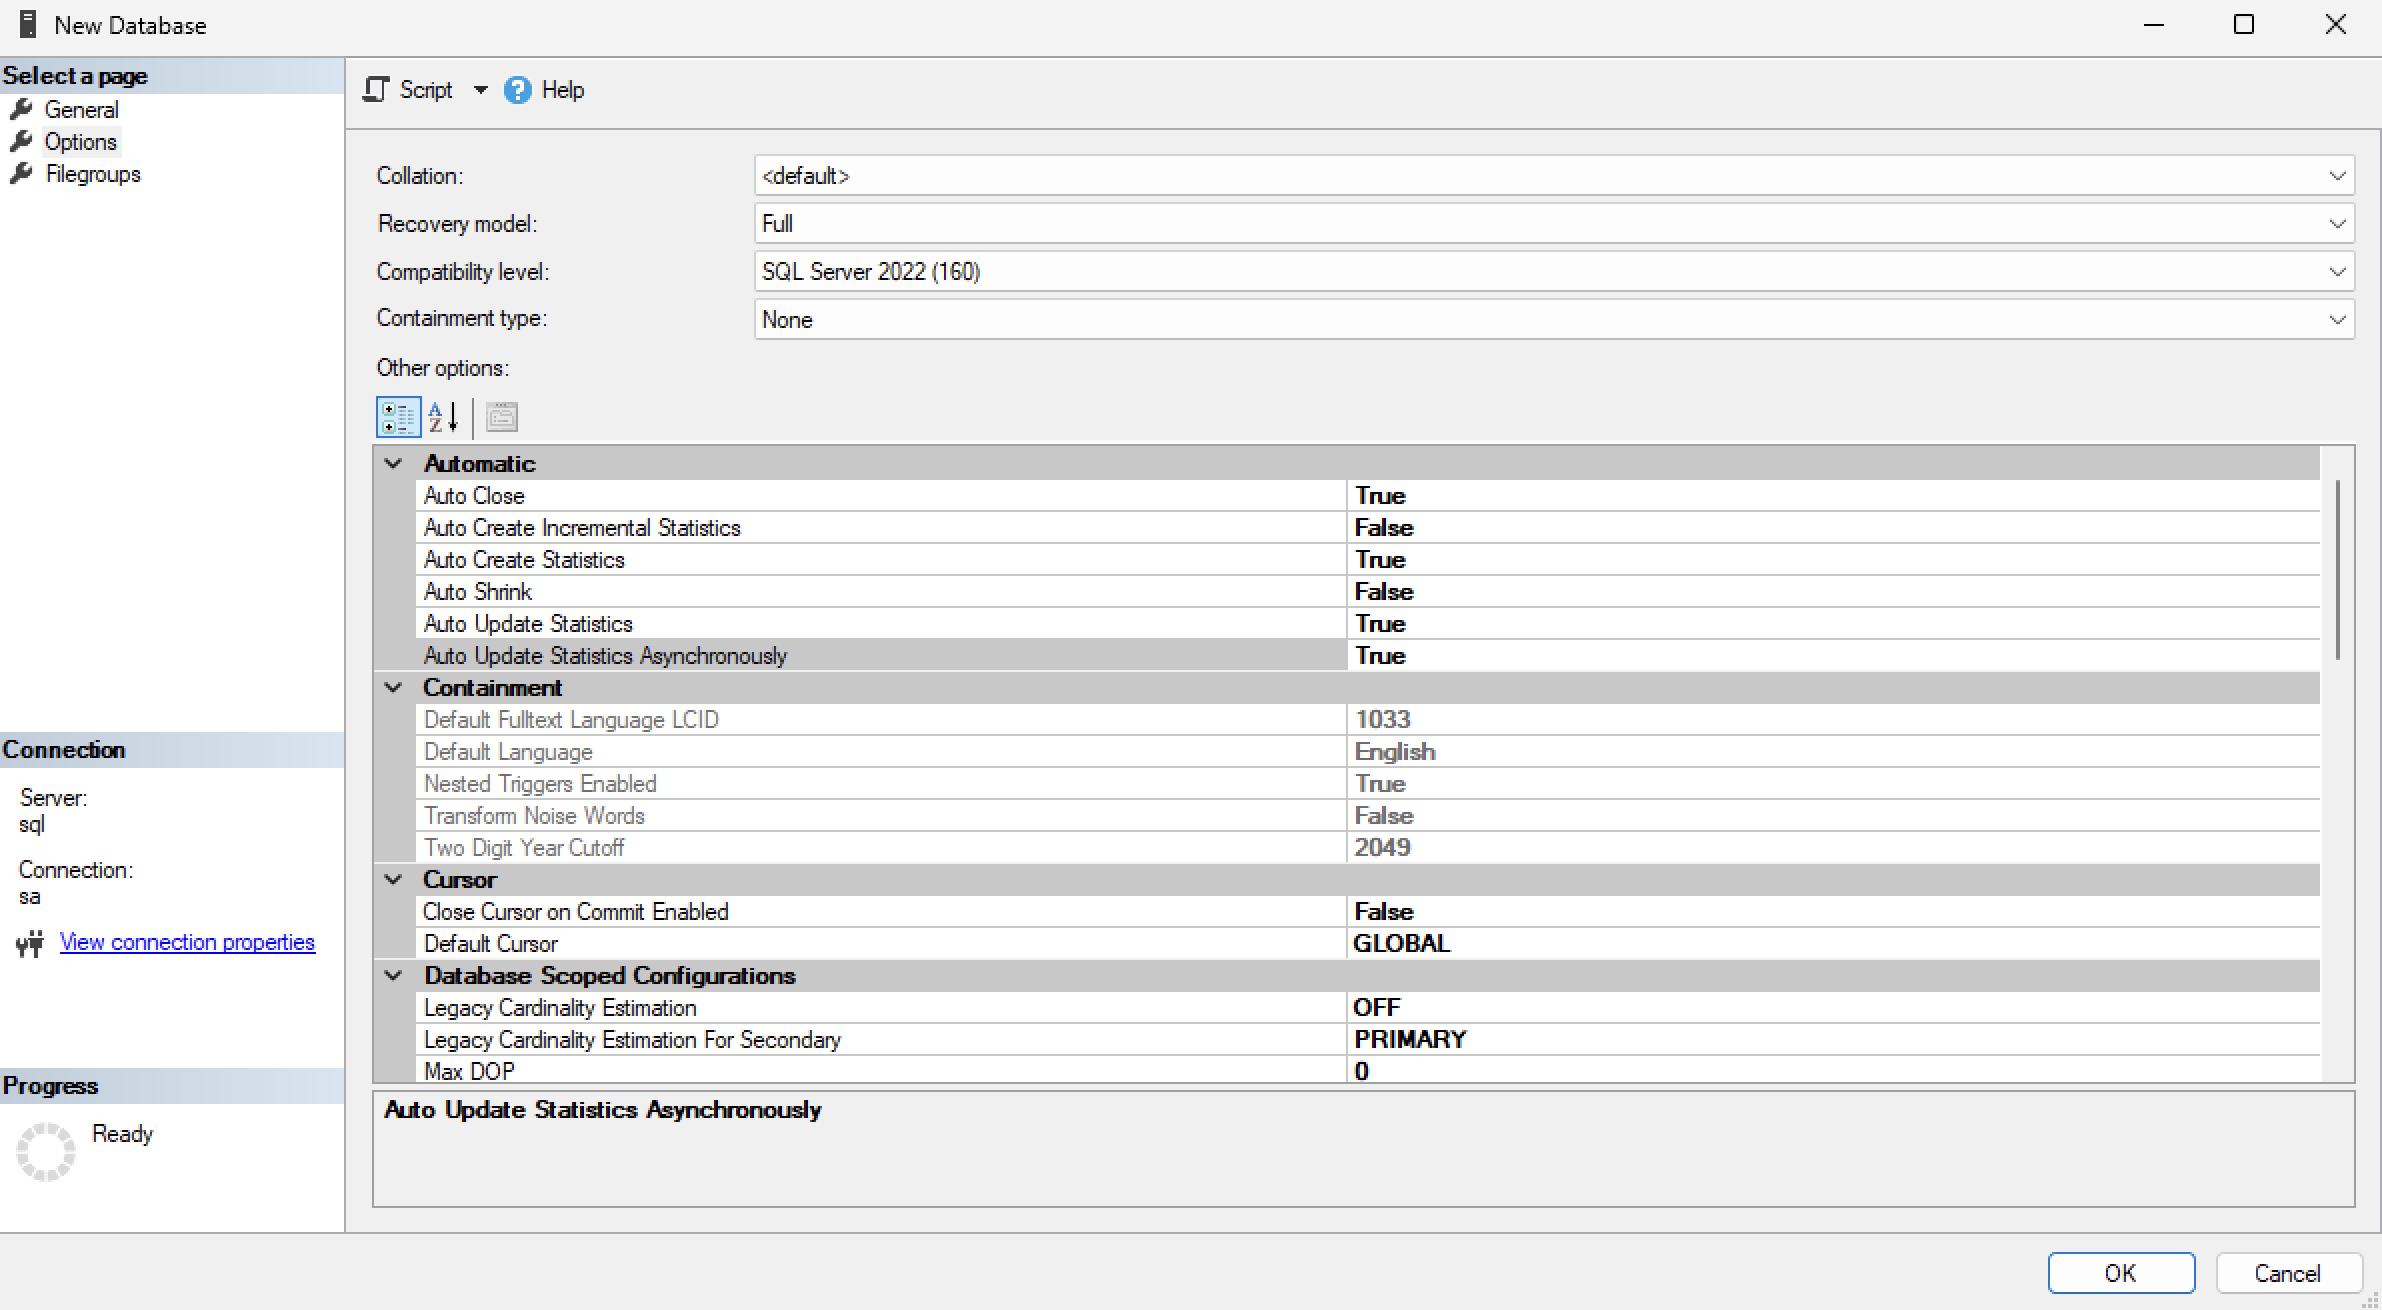
\includegraphics[width=\textwidth]{images/task-1/step-4.png}
  \caption{Настройка параметров базы данных}
  \label{fig:task-1/step-4.png}
\end{figure}

\subsubsection{Проверка создания базы данных}

После настройки параметров была нажата кнопка <<ОК>>. На рисунке
\ref{fig:task-1/step-5.png} видно, что база данных <<ApressFinancial>> была
успешно создана и готова к работе.

\begin{figure}[H]
  \centering
  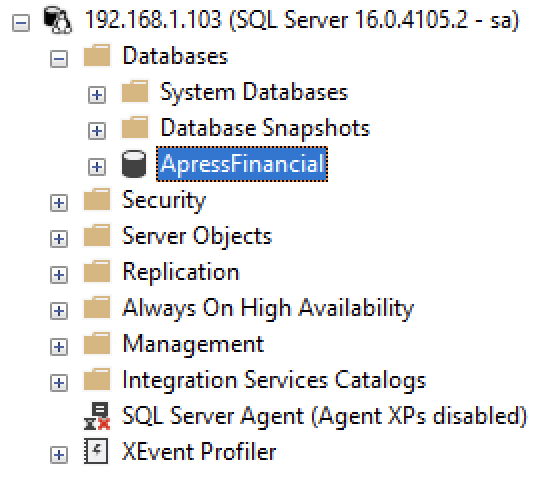
\includegraphics[width=0.5\textwidth]{images/task-1/step-5.png}
  \caption{Созданная база данных <<ApressFinancial>> в узле <<Databases>>}
  \label{fig:task-1/step-5.png}
\end{figure}

\subsection{Вторая задача}

\subsubsection{Генерация сценария создания базы данных}

С помощью контекстного меню, которое показано на рисунке
\ref{fig:task-2/step-1.png}, было открыто окно, в котором отображается
сгенерированный код с инструкциями T-SQL. Эти инструкции создают базу данных,
настроенную в предыдущих шага. Код, полученный в результате генерации, показан
на рисунке \ref{fig:task-2/step-2.png}.

\begin{figure}[H]
  \centering
  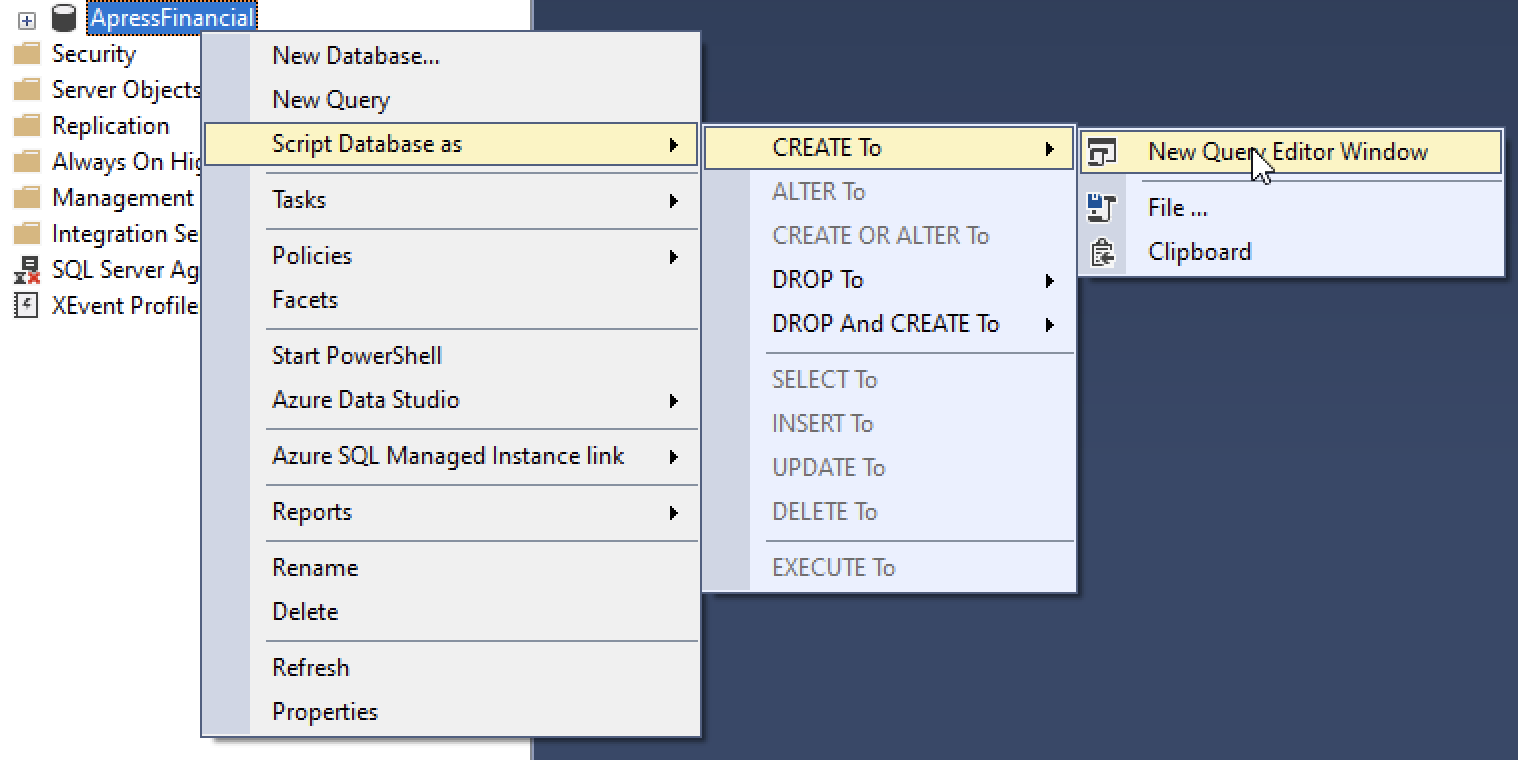
\includegraphics[width=\textwidth]{images/task-2/step-1.png}
  \caption{Открытие окна <<Query Editor>>}
  \label{fig:task-2/step-1.png}
\end{figure}

\begin{figure}[H]
  \centering
  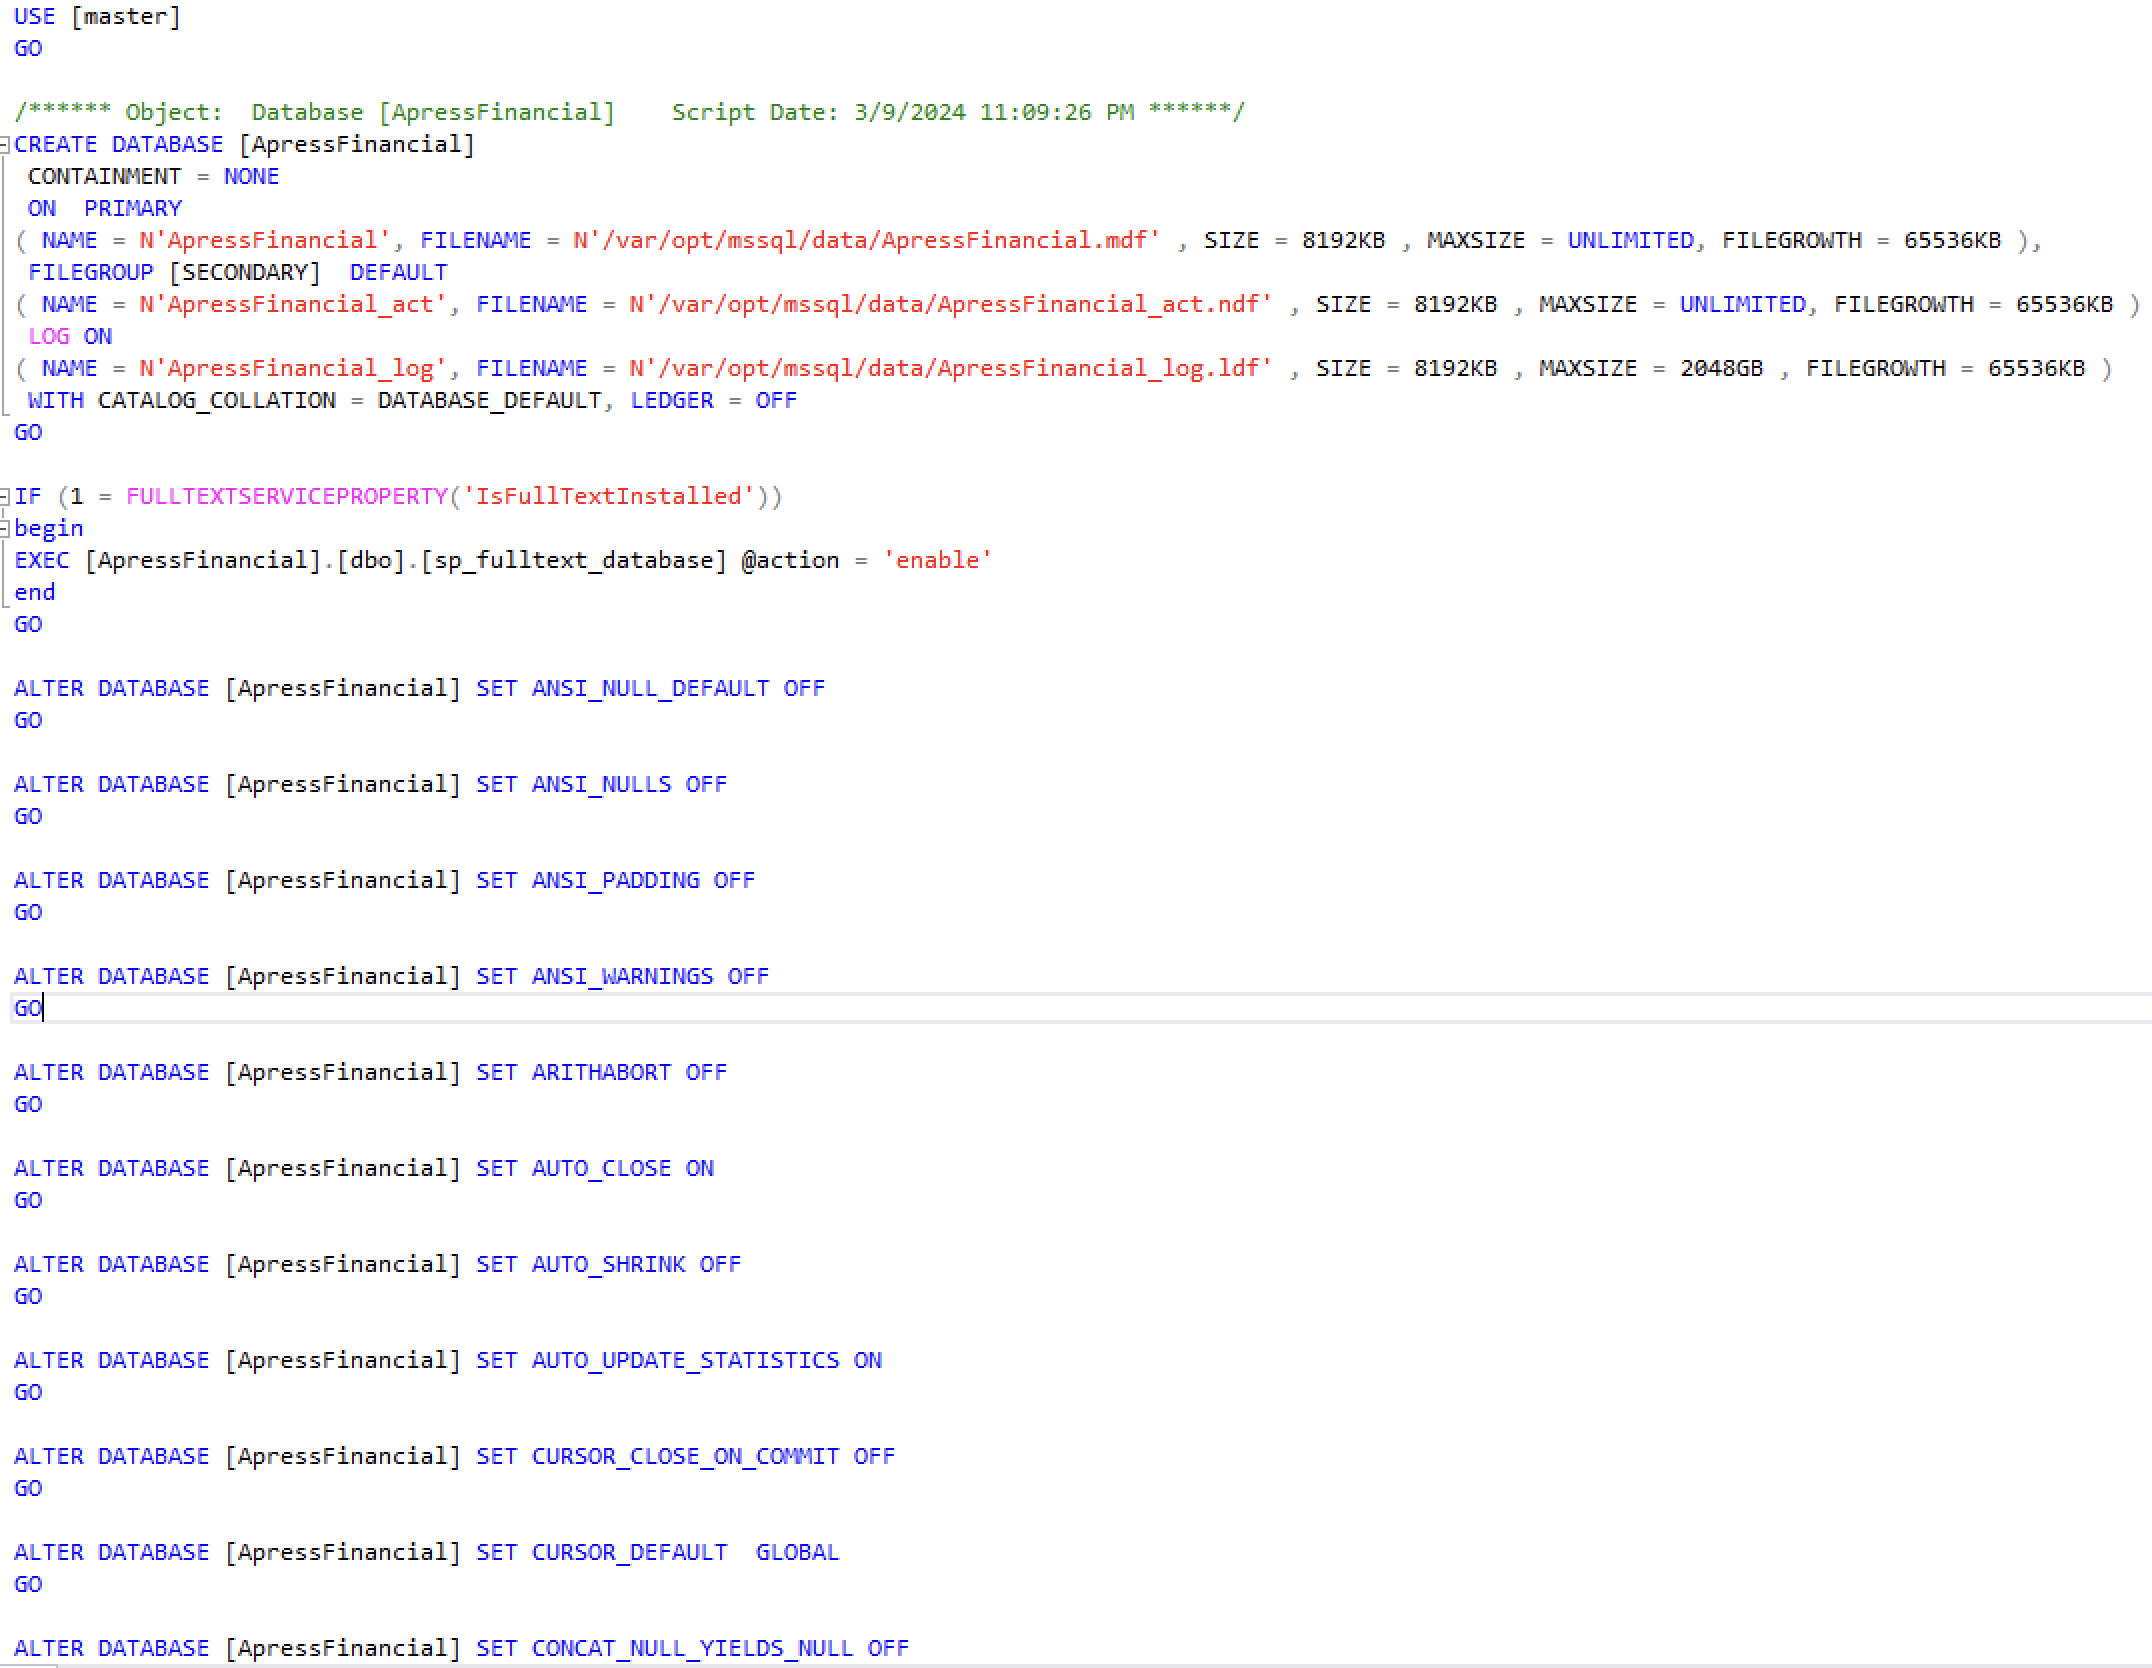
\includegraphics[width=\textwidth]{images/task-2/step-2.png}
  \caption{Сгенерированный запрос}
  \label{fig:task-2/step-2.png}
\end{figure}

\subsubsection{Анализ сгенерированного кода}

В ходе анализа сгенерированного кода выявлено, что инструкции, изображенные на
рисунке \ref{fig:task-2/step-3.png} отвечают за создание файловых групп. На
рисунке \ref{fig:task-2/step-4.png} показаны инструкции, которые устанавливают
параметры из группы <<Automatic>>.

\begin{figure}[H]
  \centering
  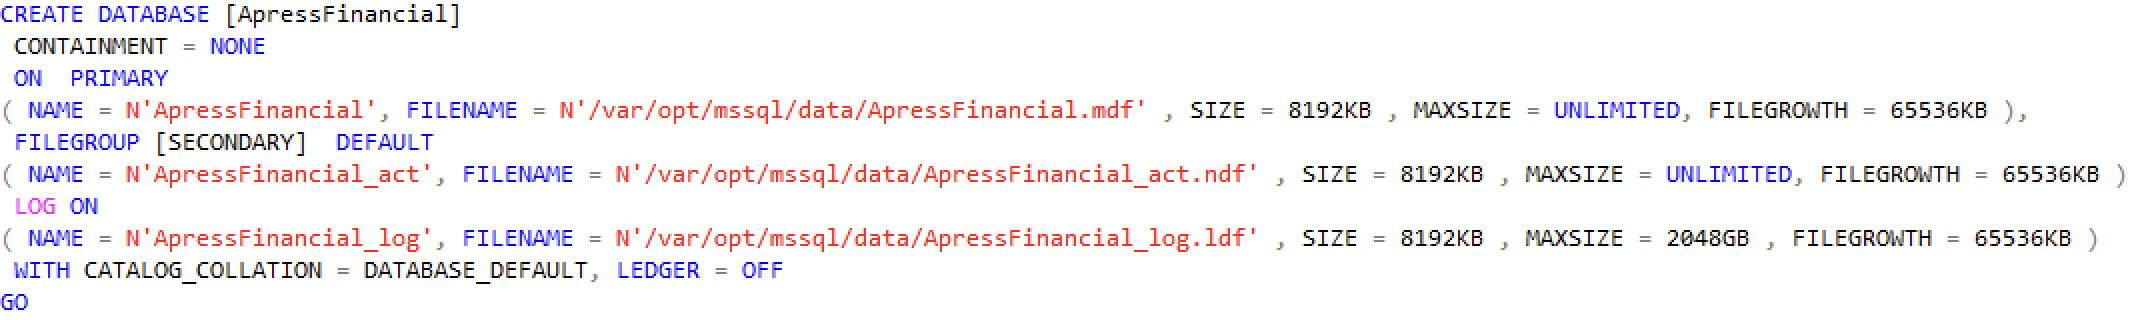
\includegraphics[width=\textwidth]{images/task-2/step-3.png}
  \caption{Место в сгенерированном коде, где создаются файловые группы}
  \label{fig:task-2/step-3.png}
\end{figure}

\begin{figure}[H]
  \centering
  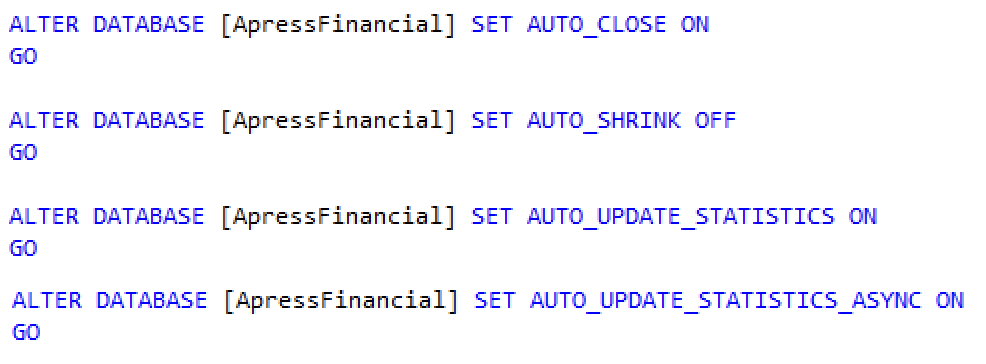
\includegraphics[width=\textwidth]{images/task-2/step-4.png}
  \caption{
    Место в сгенерированном коде, где устанавливаются параметры из группы
    <<Automatic>>
  }
  \label{fig:task-2/step-4.png}
\end{figure}

\subsection{Третья задача}

\subsubsection{Удаление базы данных}

С помощью контекстного меню, которое изображено на рисунке
\ref{fig:task-3/step-1.png}, было открыто окно удаления базы данных. Оно, в свою
очередь, показано на рисунке \ref{fig:task-3/step-2.png}. В данном окне был
выбран флажок <<Delete backup and restore history information for databases>>, а
также флажок <<Close existing connections>>. После нажатия на кнопку <<ОК>> база
данных была удалена.

\begin{figure}[H]
  \centering
  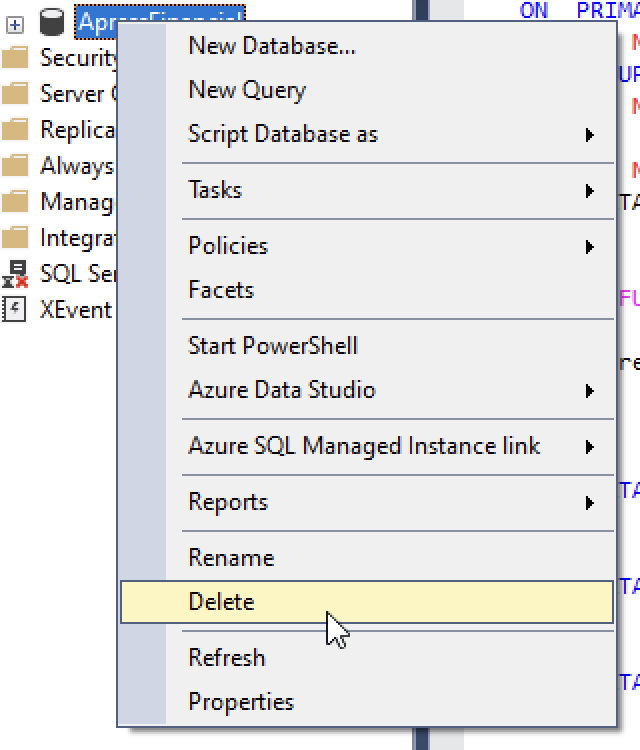
\includegraphics[width=0.5\textwidth]{images/task-3/step-1.png}
  \caption{Открытие окна удаления базы данных}
  \label{fig:task-3/step-1.png}
\end{figure}

\begin{figure}[H]
  \centering
  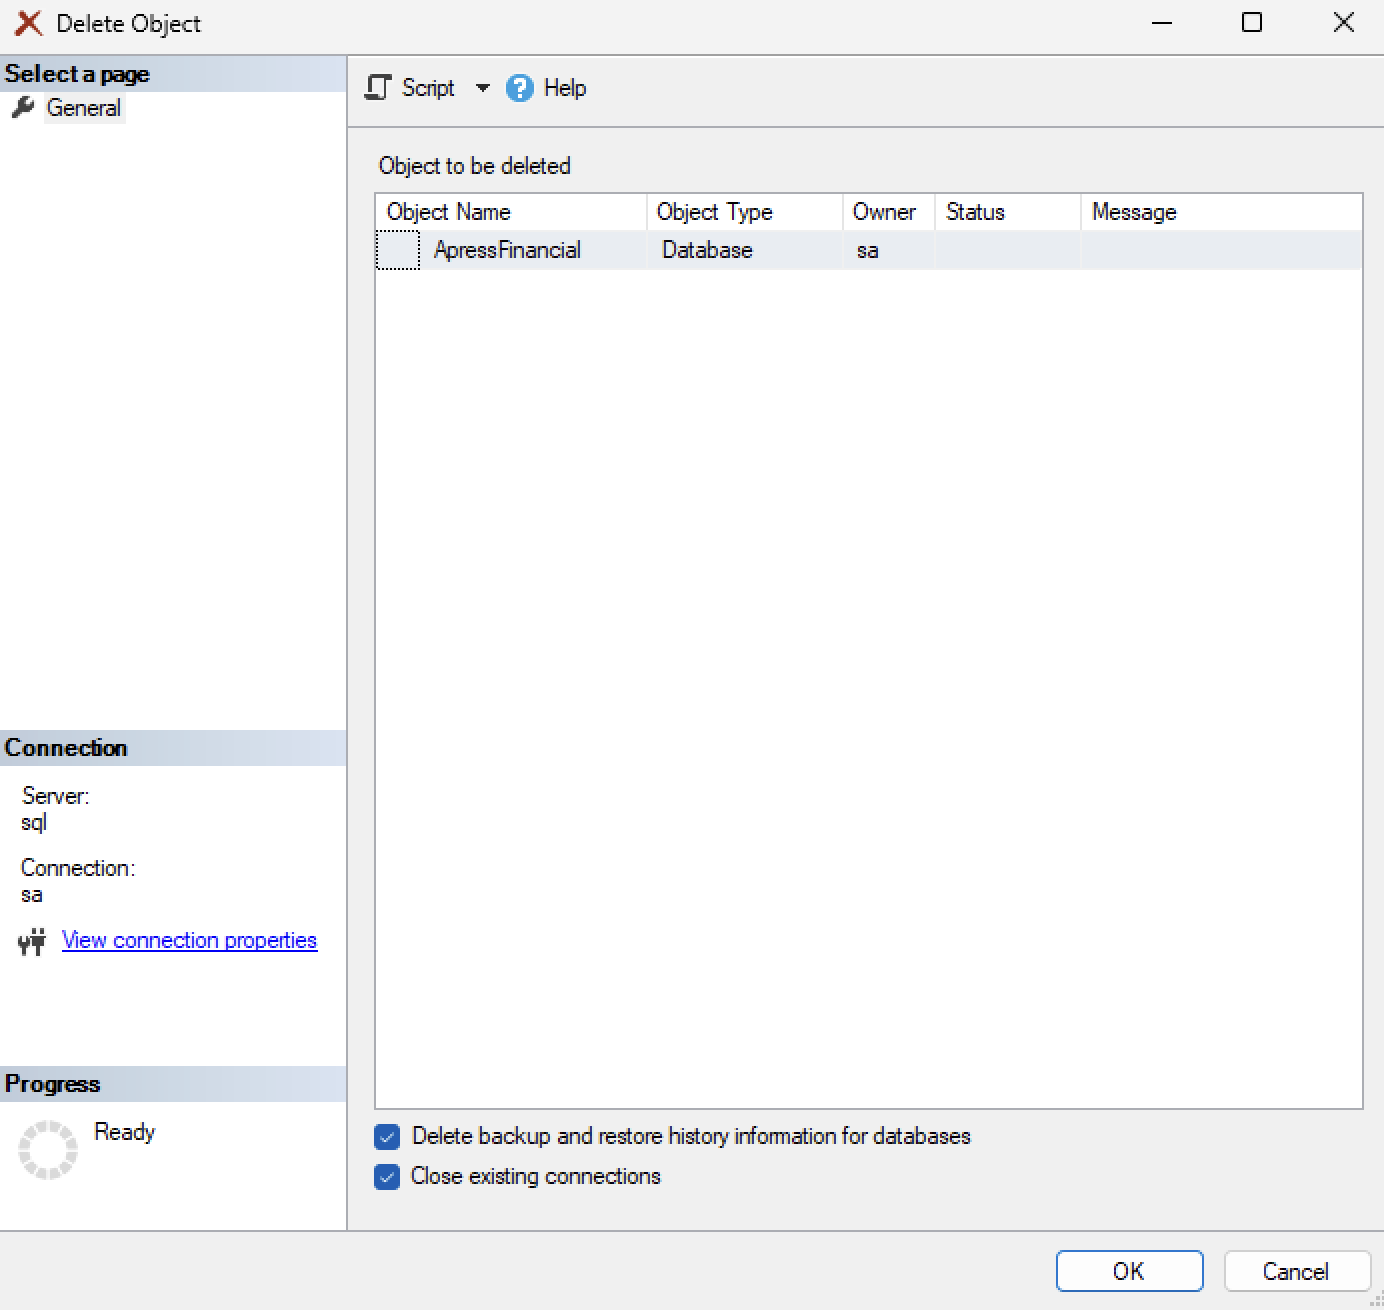
\includegraphics[width=\textwidth]{images/task-3/step-2.png}
  \caption{Окно удаления базы данных}
  \label{fig:task-3/step-2.png}
\end{figure}

\subsection{Четвертая задача}

\subsubsection{Ввод и выполнение запроса}

С помощью кнопки <<New Query>>, показанной на рисунке
\ref{fig:task-4/step-1.png} был открыт редактор запросов. После этого в редактор
был введет запрос, изображенный на рисунке \ref{fig:task-4/step-2.png}.

\begin{figure}[H]
  \centering
  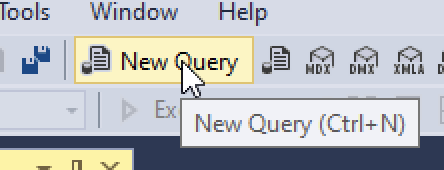
\includegraphics[width=0.5\textwidth]{images/task-4/step-1.png}
  \caption{Открытие редактора запросов}
  \label{fig:task-4/step-1.png}
\end{figure}

\begin{figure}[H]
  \centering
  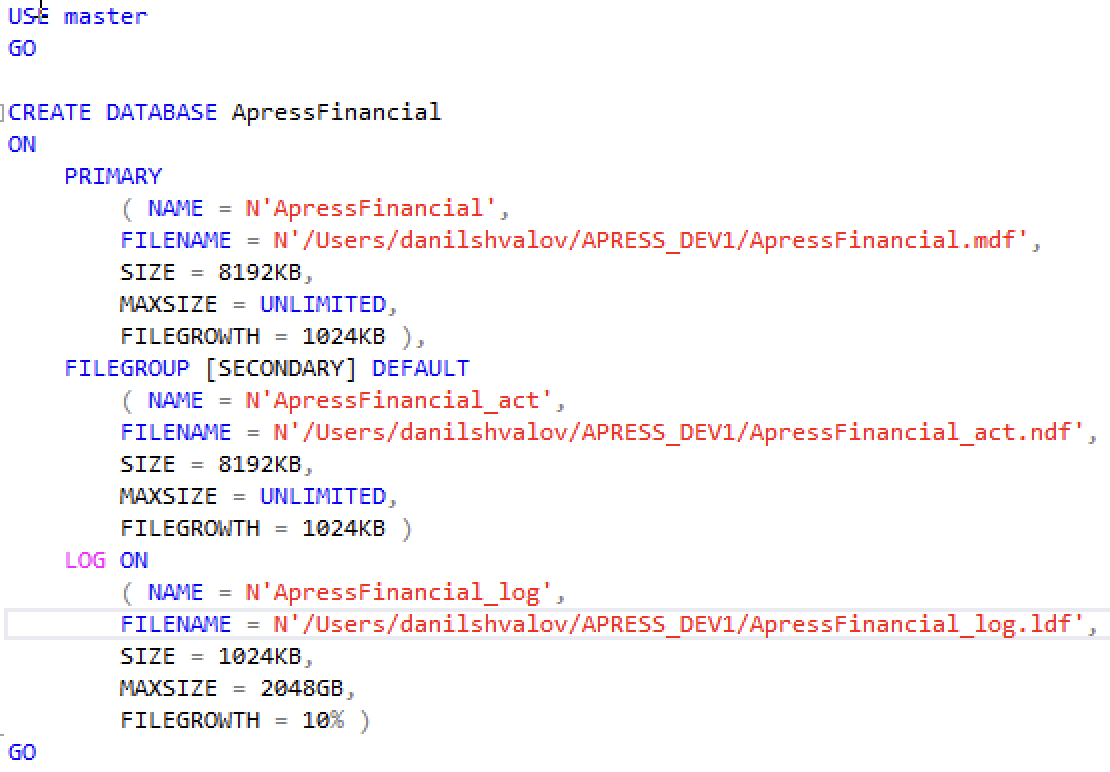
\includegraphics[width=\textwidth]{images/task-4/step-2.png}
  \caption{Запрос для создания базы данных}
  \label{fig:task-4/step-2.png}
\end{figure}

\subsubsection{Проверка создания базы данных}

После выполнения запроса, который был приведен на предыдущем шаге, в боковом
меню появилась новая база данных. Это можно увидеть на рисунке
\ref{fig:task-4/step-3.png}.

\begin{figure}[H]
  \centering
  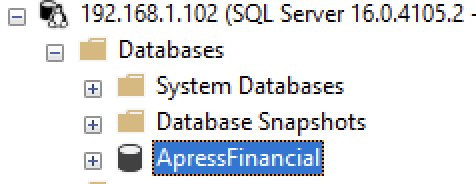
\includegraphics[width=0.4\textwidth]{images/task-4/step-3.png}
  \caption{Созданная база данных}
  \label{fig:task-4/step-3.png}
\end{figure}

\subsubsection{Настройка базы данных}

Для настройки параметров сортировки символьных строк был использован запрос,
показанный на рисунке \ref{fig:task-4/step-4.png}.

\begin{figure}[H]
  \centering
  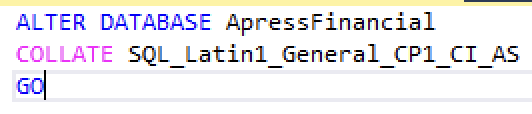
\includegraphics[width=0.7\textwidth]{images/task-4/step-4.png}
  \caption{Настройка параметров сортировки символьных строк}
  \label{fig:task-4/step-4.png}
\end{figure}

\subsection{Пятая задача}

\subsubsection{Создание схемы}

На панели инструментов была найдена папка <<Schemas>> (рисунок
\ref{fig:task-5/step-1.png}). С помощью контекстного меню, показанного на
рисунке \ref{fig:task-5/step-2.png}, было открыто окно для создания новой схемы.
Оно, в свою очередь, показано на рисунке \ref{fig:task-5/step-3.png}. После
этого в поле <<Schema Name>> было введено имя <<CustomerDetails>>.

\begin{figure}[H]
  \centering
  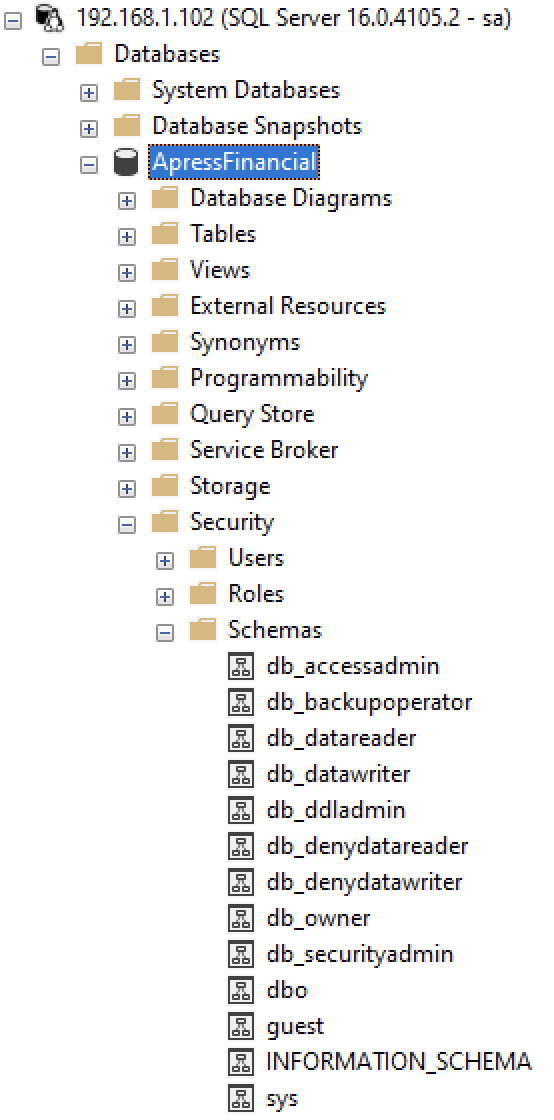
\includegraphics[width=0.5\textwidth]{images/task-5/step-1.png}
  \caption{Папка <<Schemas>>}
  \label{fig:task-5/step-1.png}
\end{figure}

\begin{figure}[H]
  \centering
  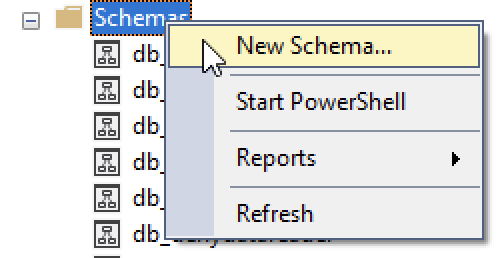
\includegraphics[width=0.4\textwidth]{images/task-5/step-2.png}
  \caption{Открытие окна создания новой схемы}
  \label{fig:task-5/step-2.png}
\end{figure}

\begin{figure}[H]
  \centering
  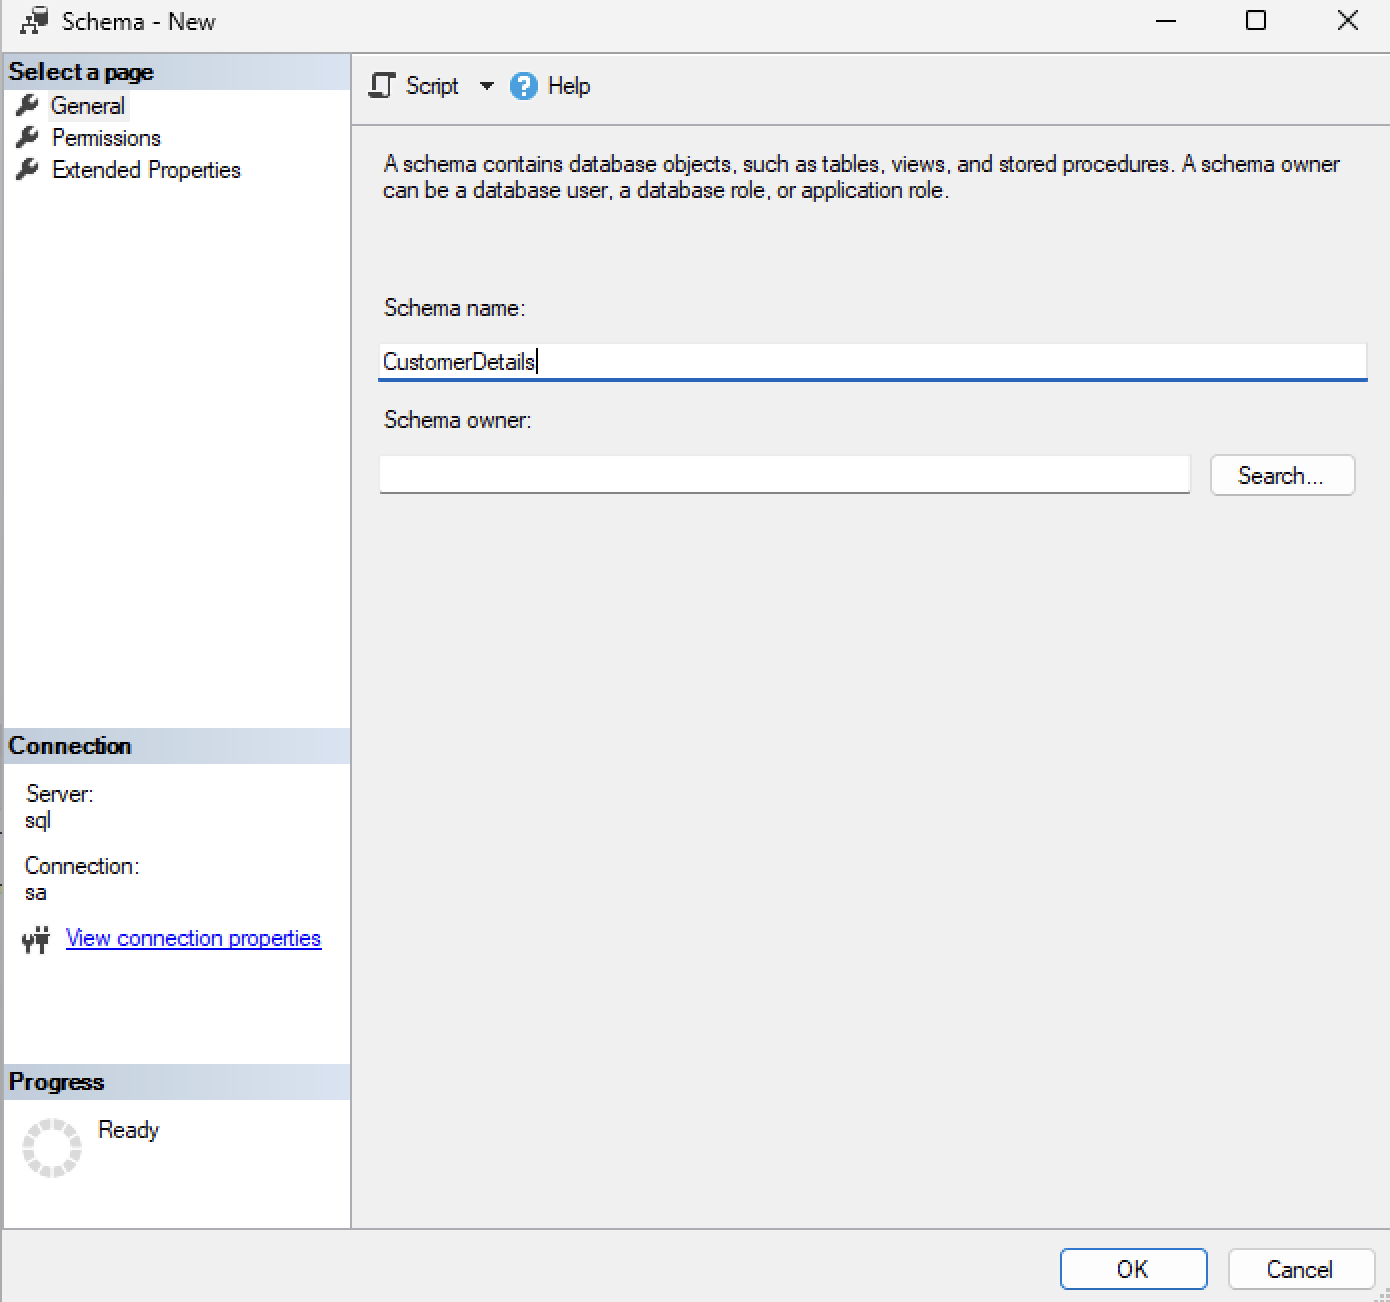
\includegraphics[width=\textwidth]{images/task-5/step-3.png}
  \caption{Окно создания новой схемы}
  \label{fig:task-5/step-3.png}
\end{figure}

\subsubsection{Проверка создания схемы}

После нажатия на кнопку <<OK>> была создана схема, что показано на рисунке
\ref{fig:task-5/step-4.png}.

\begin{figure}[H]
  \centering
  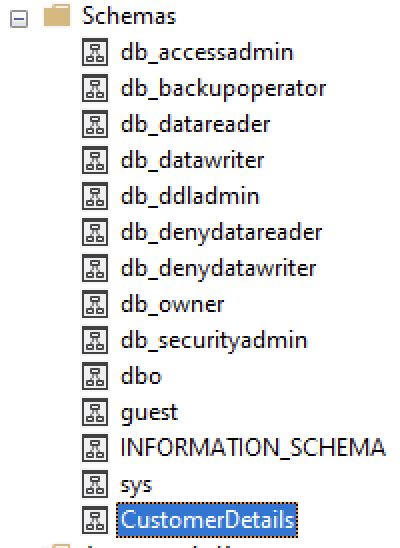
\includegraphics[width=0.4\textwidth]{images/task-5/step-4.png}
  \caption{Созданная схема}
  \label{fig:task-5/step-4.png}
\end{figure}

\subsection{Шестая задача}

\subsubsection{Создание схемы с помощью запроса}

С помощью редактора запросов был выполнен код, изображенный на рисунке
\ref{fig:task-6/step-1.png}. После выполнения в папке <<Schemas>>, как видно на
рисунке \ref{fig:task-6/step-2.png}, появилась новая схема
<<TransactionDetails>>.

\begin{figure}[H]
  \centering
  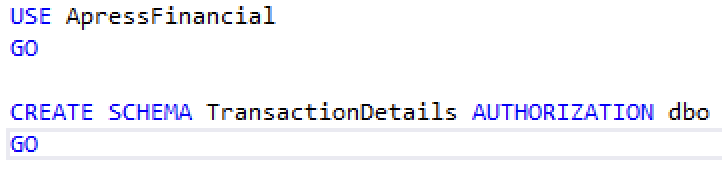
\includegraphics[width=0.8\textwidth]{images/task-6/step-1.png}
  \caption{Запрос для создания схемы <<TransactionDetails>>}
  \label{fig:task-6/step-1.png}
\end{figure}

\begin{figure}[H]
  \centering
  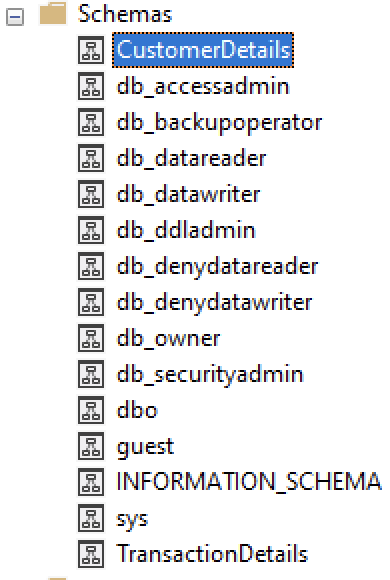
\includegraphics[width=0.4\textwidth]{images/task-6/step-2.png}
  \caption{Созданная схема}
  \label{fig:task-6/step-2.png}
\end{figure}

\section{Выводы и анализ результатов работы}

В входе выполнения лабораторной работы были изучены методы создания, изменения,
удаления баз данных и схем СУБД Microsoft SQL Server в интегрированной среде
управления базами данных Microsoft SQL Server Management Studio (SSMS).

\section{Пример решения для PostgreSQL}

\subsection{Создание базы данных}

На рисунке \ref{fig:postgres-create-database} приведен пример создания базы
данных в PostgreSQL.

\begin{code}
  \begin{minted}{sql}
    CREATE DATABASE ApressFinancial;
  \end{minted}
  \caption{Создание базы данных в PostgreSQL}
  \label{fig:postgres-create-database}
\end{code}

\subsection{Удаление базы данных}

На рисунке \ref{fig:postgres-delete-database} приведен пример удаления базы
данных в PostgreSQL.

\begin{code}
  \begin{minted}{sql}
    DROP DATABASE ApressFinancial;
  \end{minted}
  \caption{Создание базы данных в PostgreSQL}
  \label{fig:postgres-delete-database}
\end{code}

\subsection{Создание схемы}

На рисунке \ref{fig:postgres-create-schema} приведен пример создания схемы в
PostgreSQL.

\begin{code}
  \begin{minted}{sql}
    CREATE SCHEMA CustomerDetails;
  \end{minted}
  \caption{Создание схемы в PostgreSQL}
  \label{fig:postgres-create-schema}
\end{code}

\end{document}
